\documentclass[11pt]{article}

\usepackage[british]{babel} % Use British English
\usepackage[onehalfspacing]{setspace} % Increase line spacing
\usepackage[margin=2.5cm]{geometry} % Modify margins

\usepackage[hidelinks]{hyperref}
\usepackage{graphicx,booktabs,apacite} % Packages for 
\usepackage{amssymb}
\usepackage{eurosym}
\usepackage{amsmath}
\usepackage{placeins}

\usepackage{caption}
\usepackage{subcaption}
\usepackage{algpseudocode}
\usepackage{algorithm}
\usepackage{multirow}
\usepackage{booktabs}
\usepackage{siunitx}
\usepackage{comment}
\usepackage{rotating}
\usepackage{adjustbox}
\textwidth 16.8cm \topmargin -1.5cm \oddsidemargin 0cm
\evensidemargin 0cm \textheight 23.5cm \headsep 0.7cm
\begin{document}

\begin{titlepage}

\title{     

\normalsize \textsc{Seminar in Financial Case Studies}
		\\ [2.0cm]
		 \\
		\LARGE \textbf{Comparative Analysis of Probability of Default Modelling under Bayesian and Frequentist Approaches: A (Reverse) Stress Testing Perspective} % Bayesian vs. Frequentist Methods in Probability of Default Modelling and (Reverse) Stress Testing
		\\ [0.5cm]
		\normalsize \today \vspace*{5\baselineskip}}

\date{}

\author{    
		Group D: \\
		Chenyan Yang, Liu Nuo Su, \\
		Willem Castelijns, Cenchen Zhao, \\ 
		\\ 
		Erasmus University Rotterdam \\ [5.0cm]
		}

\maketitle

\thispagestyle{empty}
\end{titlepage}


\maketitle

\tableofcontents

\pagebreak
\begin{abstract}
In this paper we develop a Bayesian Hierarchical logit model to estimate the probabilities of defaults (PD) for companies in a bank's Small- and Medium-sized Enterprises portfolio. This portfolio contains a wide range of firm characteristics and is extended with macroeconomic variables in order to perform a stress test. The portfolio is stressed using the stress test scenarios provided by the European Banking Authority (EBA) for the years 2023 to 2025. For the analyzed dataset, the Bayesian Hierarchical model outperformed a traditional frequentist logistic regression model in terms of detecting default observations for the out-of-sample periods of 2016 to 2022. We show that the model is able to reproduce realistic default ratios, and credible intervals are established in the stress tests using the Bayesian properties of the model. Applying the PD model to the adverse stress test scenario designed by the EBA showed that the bank is vulnerable, as its Risk Weighted Assets increases by more than 20\%. The most important drivers for the PD are identified, and are used to create a reverse stress test scenario where Italy suffers from a debt crisis.  
%constant firm char
%baseline higher oos estimates
%reverse stress test: shock italy simulated dept crisis gdp affected, interest rate largest effect on rwa metho how macroecono condi
% and due to the Bayesian nature can also include confidence bounds on development of the defaults under the stress test scenario. 
\end{abstract}
%\section{Introduction} \label{introduction}
The market for ultra short tenor has grown tremendously in recent years. Since the introduction of the so-called 'weeklies', investors and traders have gained the ability to hedge against, or take advantage of short-term market trends and specific events without committing to longer-term contracts. In 2022, it is estimated that around 60\% of the daily option trading volume belonged to the ultra short term tenor options.  %[Introduction, grab attention]

Although making up the majority of the trading volume, limited research has been done on ultra short tenor options. For longer maturity derivative, researches modeling the Implied Volatility Surface (IVS) were often centered around the fundamentals of a company and the macro-economic trends at the time (e.g. \citeA{YAN2011216}, \citeA{bernales2014can}). For those derivatives, out-of-the money options are less affected by sudden market events, as volatility tends to stabilize over longer time horizons. In contrast, ultra short tenor options tend to expire within immediate market conditions, where the sudden volatility spike often ends up determining the payoff of the derivative. Therefore, ultra short tenor options are much more affected by immediate market conditions, making the predictability of the derivative much more challenging.
%such as spontaneous changes in market sentiment, earning announcements of a company, or news events. 
%In contrast, ultra short tenor options are much m
% smoothing? [IVS - and limited explain-ability in data[Describe the problem, IVS and thing]]

%[Quarterly numbers do not reflect the immediate market conditions]

In this work, we investigate the implied volatility of ultra short tenor options, and plot the options against different strike prices and times to maturity using the IVS. We employ machine learning algorithms, as they are suited for capturing complex, non-linear relations in the process of implied volatility estimation. Furthermore, as quarterly numbers do not immediately reflect the current market conditions, we incorporate news data obtained from The New York Times as explored by \cite{kim2023forecasting} as input. We make use of the FinBERT language model developed by \cite{yang2020finbert}, and is specialized to obtain the semantics of the text, use the embedding, and transform them into a format compatible for machine learning for Financial news data. 


%The price of an option is usually expressed in terms of implied volatility, as the one-to-one mapping allows for comparison of options across different strike prices and times to maturity. Plotting the volatility against the two results in the well-known IVS used by practitioners and researches alike.  %IVS here

%Furthermore, we [text data, FinBERT embedding]
%[you see them reading the news all the time]

%[machine learning]

%[Describe idea, and approach to problem - text data and Machine learning]




%[Academic and economic relevance]
From an academic standpoint, we contribute to literature investigating ultra short tenor options. We demonstrate the use of text, and we employ state of the art machine learning techniques in the context of short tenor derivatives. From an economic standpoint, the IVS is used to gauge the market sentiment at the time, and the inclusion of text data can reveal the relation between specific news events and the sentiment at the time. 

%[Research question]

In this work,  we aim to answer the following questions:
1. How useful is news data in the prediction of implied volatility surfaces of ultra short tenor options?

2. To what extend can machine learning algorithms predict the implied volatility surface of ultra short tenor derivatives?

3. What differences exist between the estimation of individual stock options and the S\&P500 index options?

[4. (Ideally) we want to make an improvement on one of the machine learning algorithms, too, and see if it is superior to the other algorithms]
[Short answer to questions]

%[Overview of the rest of the paper]
In section \ref{literature_review}, previous works on the IVS and short tenor options are investigated. Section \ref{Data} gives an overview of the data, while \ref{methods} discusses the methods used in this work.  




%\section{Literature Review} \label{literature_review}

[Describe gap in literature - weekly options not researched much]

Contribution to literature:
1. Investigate the IVS on ultra short tenor options
2. Demonstrate the use of machine learning methods on the estimation of implied volatility
3. Explore the use of text data to gauge the sentiment around the stocks 
%\section{Data} \label{Data}

\subsection{Ultra Short Tenor Options} \label{3_ultra_short_tenor}
[Graphs and trends in data]

\begin{figure}
    \centering
    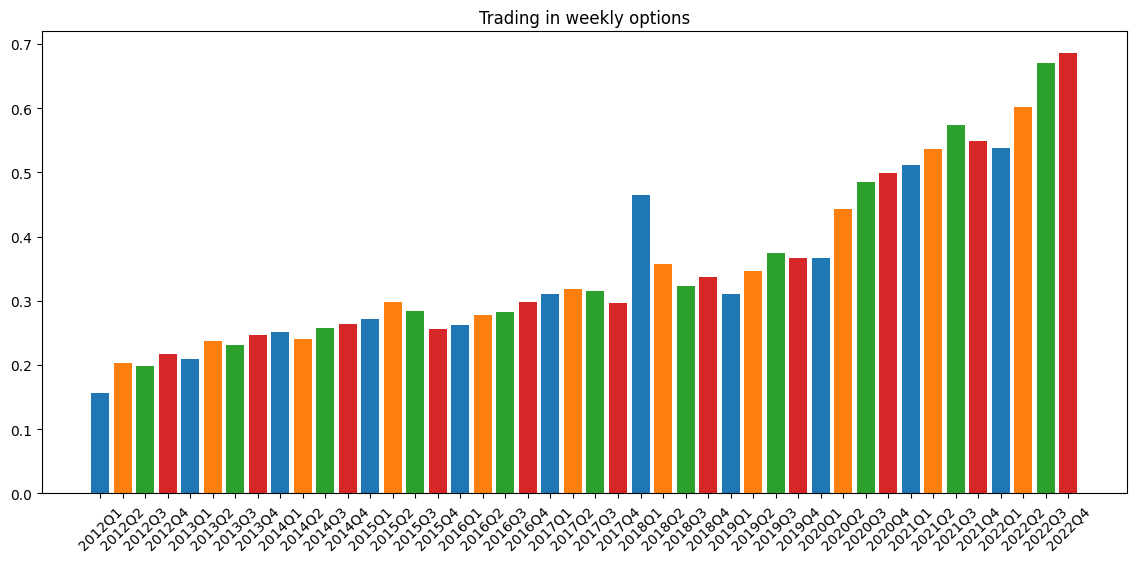
\includegraphics[width=\linewidth]{report/option_volume.png}
    \caption{Caption}
    \label{fig:enter-label}
\end{figure}
First: options data
time period, maturities, 

S\&P500 first, then individual stocks

\subsection{Macro Economic Variables and Events} \label{3_macro_data}
Second: Macro-economic variables 
Third: News and text data - FinBERT - demonstrate the embeddings

\subsection{Idiosyncratic Variables and News} \label{3_stock_data}

Then, singular stock options
- accounting variables ?
%\input{4_methodology}
%\input{5_results}
%\input{6_conclusion}



%Pre-variable selection: Logistic regression: Correlation matrix, Stepwise regression based on AIC, BIC; ML: LASSO; Principle Component Analysis

%Data: Macro variables of every country, same as for the stress scenario: GDP, unemployment rate, inflation


\newpage
\bibliographystyle{apacite}
\bibliography{bibliography}
\newpage
%\input{Appendix}


\end{document}
